\documentclass[12pt,a4paper, oneside,ngerman]{scrartcl}
\usepackage[ngerman]{babel}			% deutsche Namen/Umlaute
\usepackage[utf8]{inputenc}			% Zeichensatzkodierung
\usepackage{graphicx}				% Einbinden von Bildern
\usepackage{color}				% Farben wenn es sein muß
\usepackage{eurosym}
\usepackage[T1]{fontenc}
\usepackage{amssymb,amsmath,amsthm, mathtools}
\usepackage{dsfont}
\usepackage{algorithm}
\usepackage{algpseudocode}
\usepackage{pstricks-add}
\usepackage{units}
\usepackage{textcomp}
\usepackage{subfigure}
\usepackage{mwe} % new package from Martin scharrer
\usepackage{caption}
\usepackage{hyperref} 
\usepackage{float}
%\usepackage[figure]{hypcap} 

\bibliographystyle{unsrt}
\setlength{\parindent}{0pt}%gegen Einrücken nach Bildern



\subject{Abschlussbericht im Rahmen des
Studienprojekts Technomathematik 2015/2016 (Bachelor) TU Dortmund}
\title{\large{Technische-, numerische- und Implementierungsaspekte des Designs einer Niedrigenergie-HPC-Plattform für den Betrieb durch erneuerbare Energien}}
%\subtitle{\small{Studiengang Technomathematik, Bachelor Lehrstuhl für Angewandte Mathematik und Numerik (LS3) Fakultät für Mathematik, TU Dortmund}}
\publishers{Vorgelegt von: Dario Jansen, Heiko Poelstra, Enno Tiemann, Kevin Hollmann, Justus Altmeyer, Daniel Tomaschewski, Marius Milcarek, Simon Vogel,  Thomas Helmich, Micha Weimann, Christoph Maria Höppke, David Schneider, Jonas Dünnebacke
\parbox[b][8cm]{\textwidth}{\centering Betreuer: Dipl.-Inf. M. Geveler und Prof. Dr. S. Turek}}
\date{\today}


\begin{document}
\thispagestyle{empty}
\newcommand{\Rule}{\rule{\textwidth}{1mm}}
\begin{center}
\Rule\vspace{5mm}
\sffamily\bfseries\Huge
\sf Abschlussbericht
\vspace{1mm}\Rule
\vfill
\small im Rahmen des\par
\Large Studienprojekts Technomathematik 2015/2016 (Bachelor)\par TU Dortmund\par
\vfill
\small mit dem Titel:\par
\Large Technische-, numerische- und Implementierungsaspekte des\par 
Designs einer Niedrigenergie-HPC-Plattform\par für den Betrieb durch erneuerbare Energien\par
\vfill
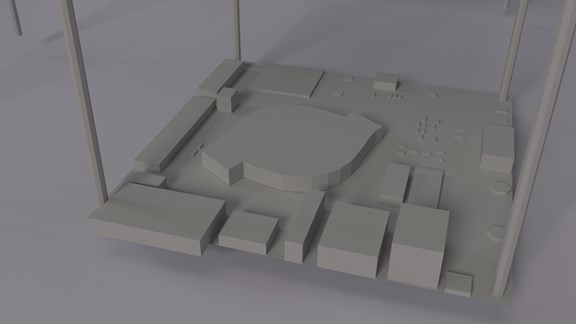
\includegraphics[width=0.6\textwidth]{Bilder/figures/render6}\par
\vfill
{\small \sf{ vorgelegt von}}\par
\vspace{1mm}
{\Large \sf {Dario Jansen, Heiko Poelstra, Enno Tiemann, Kevin Hollmann, Justus Altmeyer, Daniel Tomaschewski, Marius Milcarek, Simon Vogel,  Thomas Helmich, Micha Weimann, Christoph Maria Höppke, David Schneider, Jonas Dünnebacke}}\par
\vspace{2mm}
{\small \sf{ betreut durch}}\par
\vspace{1mm}
{\Large \sf{Dipl.-Inf. Markus Geveler}}\par
{\small \sf{ und}}\par
{\Large \sf{Prof. Dr. Stefan Turek}}\par

\vfill
{März 2016}
\end{center}
\newpage
\thispagestyle{empty}
\sf

\newpage
\tableofcontents
\newpage

\section{Motivation und Problembeschreibung}
Im Bereich des wissenschaftlichen Hochleistungsrechnen gibt es seit 1993 die \glqq TOP500 List\grqq, welche die Supercomputer, geordnet nach ihrer Leistung in Floating Point Operationen pro Sekunde auflistet. Der momentane Spitzenreiter, der Tianhe-2, erreicht dabei bei voller Auslastung einen Energieverbrauch von 155.998,08 MWh jährlich. Dieser extrem hohe Wert bedeutet gleichzeitig große Betriebskosten, welche im Zeitalter der Energiewende kaum zu rechtfertigen sind. Daher wurde als Konkurrenzobjekt im Jahr 2007 die \glqq Green500 List\grqq eröffnet, welche die Supercomputer entsprechend ihrer Rechenleistung pro Watt sortiert. Und genau an dieser setzt das Studienprojekt Technomathematik 2015/2016 der TU Dortmund an, welches begleitend zum I.C.A.R.U.S.-Projekt des Lehrstuhl 3 der Fakultät Mathematik der TU Dortmund läuft. 
Ziel ist es, die Hardware- und Softwareentwicklung eines energieeffizienten \texti{High-Performance Computing} (HPC) Systems nachzuvollziehen und zu begleiten. Grundlage dafür ist der mobile Grafikprozessor NVIDIA Tegra K1, welcher höchste Energieeffizienz verspricht und, nach dem Vorbild der Energiewende, durch Solarzellen betrieben wird. Die Nutzung dieses mobilen, auch eingebetteten Systems genannt (engl:\glqq embedded systems\grqq), erklärt sich durch die Anwendungsgebiete dieser Geräte. Sie werden in der Unterhaltungsindustrie, Automobilindustrie oder sogar als Herzschrittmacher in der Medizin eingesetzt. Diese Anwendungsbereiche verlangen ein enorm energiesparsames Verhalten, da die mobile Energiezufuhr über Batterien nicht endlos ist. Daher sind diese Systeme eine attraktive Möglichkeit beim sogenannten \texti{Green Computing}.
Das Hochleistungsrechnen spielt in der Mathematik eine große Rolle, da Differentialgleichungen Naturvorgänge verschiedener Art, wie zum Beispiel Schwingungen, Wellenausbreitungen oder Strömungen beschreiben können. Die Lösung dieser Gleichungen erfordert einen, je nach Genauigkeit des Resultats, erheblichen numerischen Aufwand, welcher nur mit Hilfe von geeigneter Hardware erreichbar ist. Da es das Vorhaben unseres Studienprojekts ist, den Luftstrom und die Wärmeleitung um und in einem geometrischen Körper wie dem des Tegra K1-Boards zu simulieren, spielen Differentialgleichungen eine wichtige Rolle für uns. Außerdem ist es dafür wichtig, die Software nach dem Paradigma der hardware-orientierten Numerik zu konstruieren, um die Leistung des Grafikprozessors effizient auszunutzen. Dazu werden 60 der NVIDIA Boards zu drei Racks angeordnet, um den Code parallelisiert laufen lassen zu können. Man kann also im Umkehrschluss auch davon sprechen, dass die Hardware der Software angepasst wird, also \textit{software-orientierte Hardware}. 
Der Aufbau des Hauptteils des Berichts lässt sich dabei in drei große Themen gliedern. Zunächst die Hardware in seinen Einzelteilen, also die Hardwareauswahl, der Aufbau des Racks und die Energieverbrauchsmessung erklärt. Darauffolgend werden die Softwarekomponenten, welche die Assemblierung mit finiten Elementen und finiten Differenzen, sowie den Löser umfassen, erläutert. Abschließend werden verschiedene Testergebnisse, welche mit der Anordnung des Studienprojekts erzielt wurden, vorgestellt und die Rechenleistung anhand dieser Resultate bewertet. 



\section{Einleitung}


Im Bereich der hardware-orientierten Numerik wurden bereits in den vergangenen Jahren einige Untersuchungen gemacht. So wurde in den Jahren 2010 und 2011 durch Geveler et al. die Lattice-Boltzmann-Methode zur Lösung von Navier-Stokes- und Flachwassergleichungen auf unterschiedlicher Hardware analysiert. Es stellte sich heraus, dass GPUs Multi-Core CPUs mit einem Speedup von bis zu acht überlegen sind, ohne dabei an Genauigkeit der numerischen Lösung einzubü\ss en. 
In \glqq Efficient Finite Element Geometric Multigrid Solvers for Unstructured Grids on GPUs\grqq\, wurde bereits 2011 nach dem Paradigma der hardware-orientierten Numerik ein geometrisches Mehrgitterverfahren mit finiter Elemente Assemblierung entwickelt, welches nur aus einer Reihe von Sparse Matrix-Vektor Multiplikationen besteht. Durch diese Implementierung, welche keinen Leistungsverlust nach sich zog, war es möglich, die Parallelität von Rechenarchitekturen noch besser auszunutzen. Besonders durch die Verwendung von GPUs anstatt von Multi-Core CPUs ergab sich ein durchschnittlicher Speedup von 8.
Geveler et al. betrachtete 2013 in \glqq 
Towards a complete FEM-based simulation toolkit on GPUs: Geometric Multigrid solver\grqq\, die Lösung partieller Differentialgleichungen mit finiten Elementen und Mehrgitterverfahren auf unstrukturierten Gittern. Es wurde gezeigt, dass sich die Laufzeit der Anwendung erheblich verbessern lässt, sobald GPUs anstatt von Multi-Core CPUs benutzt wurden. 
Des Weiteren wurde in \glqq Energy efficieny vs. Performance of the numerical solution of PDEs: An application study on a low-power ARM-based cluster\grqq\, ein Cluster aus 96 ARM Cortex-A9 Dual-Core Prozessoren einer Rechenarchitektur, basierend auf x86-Prozessoren gegenüber gestellt. Dabei wurde die verbrauchte Energie zur Lösung von drei wissenschaftlichen Anwendungen, einem Finite-Elemente Code mit Mehrgitter-Löser, einer strömungsmechanischen Anwendung und einem Code zur Ausbreitung von Schallwellen mit Hilfe der Spektral-Elemente Methode, analysiert. Schließlich wurde gezeigt, dass die verbrauchte Energie zur Lösung erheblich gesenkt werden kann, im Einklang mit einer akzeptablen Erhöhung der Laufzeit. 
In \glqq Porting FEASTFLOW to the Intel Xeon Phi: Lessons Learned\grqq\, zeigte Geveler et al. die Leistungsverbesserung von axpy-Vektor Operationen und Sparse Matrix-Vektor Multiplikationen durch Nutzung des Intel Xeon Phi Koprozessors. Diese Analyse, sowie in \glqq FFF2: Future-proof High Performance Numerical Simulation for CFD with FEASTFLOW (2)\grqq\, durchgeführten Untersuchungen, welche sich mit der Entwicklung von numerischen Methoden zur parallelen Lösung von partiellen Differentialgleichungen für realitätsnahe industrielle und wissenschaftliche Probleme befassen, basierten auf der Software Infrastruktur \glqq FEASTFLOW\grqq. Dieses Paket umfasst Software zur numerischen Lösung der Navier-Stokes-Gleichungen in 2D und 3D. 

\documentclass[a4paper]{scrartcl}
\usepackage{german} 
% Damit die Verwendung der deutschen Sprache nicht ganz so umst\"andlich wird,
% sollte man die folgenden Pakete einbinden: 
%\usepackage[latin1]{inputenc}% ermöglich die direkte Eingabe der Umlaute 
\usepackage[utf8]{inputenc}
\usepackage[T1]{fontenc} % das Trennen der Umlaute
\usepackage{ngerman} % hiermit werden deutsche Bezeichnungen genutzt und 
                     % die W\"orter werden anhand der neue Rechtschreibung 
		     % automatisch getrennt.  
		     
\usepackage{amsmath, amsthm, amssymb, amsfonts}

\begin{document}

\end{document}

\section{Software}


Das als Löser verwendete Verfahren des Projektes ist das sogenannte BiCGStab-Verfahren (engl: „biconjugate gradient stabilized method“), welches zur Klasse der Krylov-Unterraum-Verfahren zählt. Diese iterative Methode wurde von H.A. van der Horst als Löser für nicht-symmetrische lineare Gleichungssysteme entwickelt und benötigt somit keine zusätzlichen Anforderungen an die Systemmatrix A wie zum Beispiel beim CG-Verfahren. Sein Name ist davon abgeleitet, dass die im nicht-vorkonditionierten Algorithmus verwendeten Residuen biorthogonal sind, also $(r_i,\hat{r}_j)=\,0$ $\forall i\neq j$, und die Suchrichtungen bikonjugiert sind bezüglich der Systemmatrix $A$, also $(Ap_i,\hat{p}_j)=\,0$ $ \forall i \neq j$.  Man entschied sich für dieses Verfahren, da das konkurrierende GMRES-Verfahren weniger speichereffizient arbeitet und das BiCGStab-Verfahren leichter zu implementieren ist.  Au\ss{}erdem kann es mit beliebigem Vorkonditionierer und ohne Vorkonditionierer implementiert werden. Der Nachteil des angewendeten Verfahrens ist, dass die Konvergenz nicht allgemein bewiesen ist. So kann es im Falle von einer Systemmatrix mit großen komplexen Eigenwerten zur Stagnation des Algorithmus kommen, ohne dass eine gute Näherungslösung ermittelt wurde. 


\begin{enumerate}
	\setlength{\itemsep}{0cm}
	\setlength{\parsep}{0cm}
	
	
	\item $r_0$=$b$-$A$$x_0$\\
	\item $\hat{r}_0$=$r_0$\\
	\item $\rho_0$=$\alpha$=$\omega_0$=1\\
	\item $v_0$=$p_0$=0\\
	\item for $i$=1,2,\dots
	\par
	\begingroup
	\leftskip=1cm 
	\noindent 
	\item$\rho_i=$\,($\hat{r_0}$,$r_{i-1}$)\\
	\item$\beta=$\,($\rho_i$/$\rho_{i-1}$)($\alpha$/$\omega{i-1}$)\\
	\item$p_i=$\,$r_{i-1}$+$\beta$($p_{i-1}-\omega_{i-1}v_{i-1}$)	\\
	\item$y=$\,$K^{-1}p_i$\\
	\item$v_i=$\,$Ay$\\
	\item$\alpha=$\,$\rho_i/(\hat{r_0},v_i)$\\
	\item$s=$\,$r_{i-1}-\alpha$$v_i$\\
	\item Wenn $\parallel s \parallel$ klein genug, setze $x_i=$\,$x_{i-1}+\alpha$$p_i$ und beende das Verfahren \\
	\item$z=$\,$K^{-1}s$\\
	\item$t=$\,$Az$\\
	\item$\omega_i=$\,$(K^{-1}_1$$t,K^{-1}_1$$s)/(K^{-1}_1$$t,K^{-1}_1$$t)$ \\
	\item$x_i=$\,$x_{i-1}+\alpha$$y+\omega_i$$z$\\
	Wenn $\parallel x-x_i \parallel < TOL $ wird das Verfahren beendet \\
	\item$r_i=$\,$s-\omega_i$$t$\\
	
	
	\par
	\endgroup 
\end{enumerate}
Der von rechts vorkonditionierte BiCGSTAB-Algorithmus startet ausgehend von einem Anfangsvektor $x_0$, welcher immer als Nullvektor implementiert wurde. Des Weiteren wurde die maximale Iterationszahl auf $10.000.000.000$ gesetzt und die Toleranz mit $TOL= 10^{-9}$ festgelegt. Der Vorkonditionierer hat dabei die allgemeine Form: 
$K = K_1 K_2 \approx A $


\section{Results}

%\section{Anhang}

\subsection{Dokumentation}
\include{refman.pdf}

\section{Anhang}

\subsection{Dokumentation}
%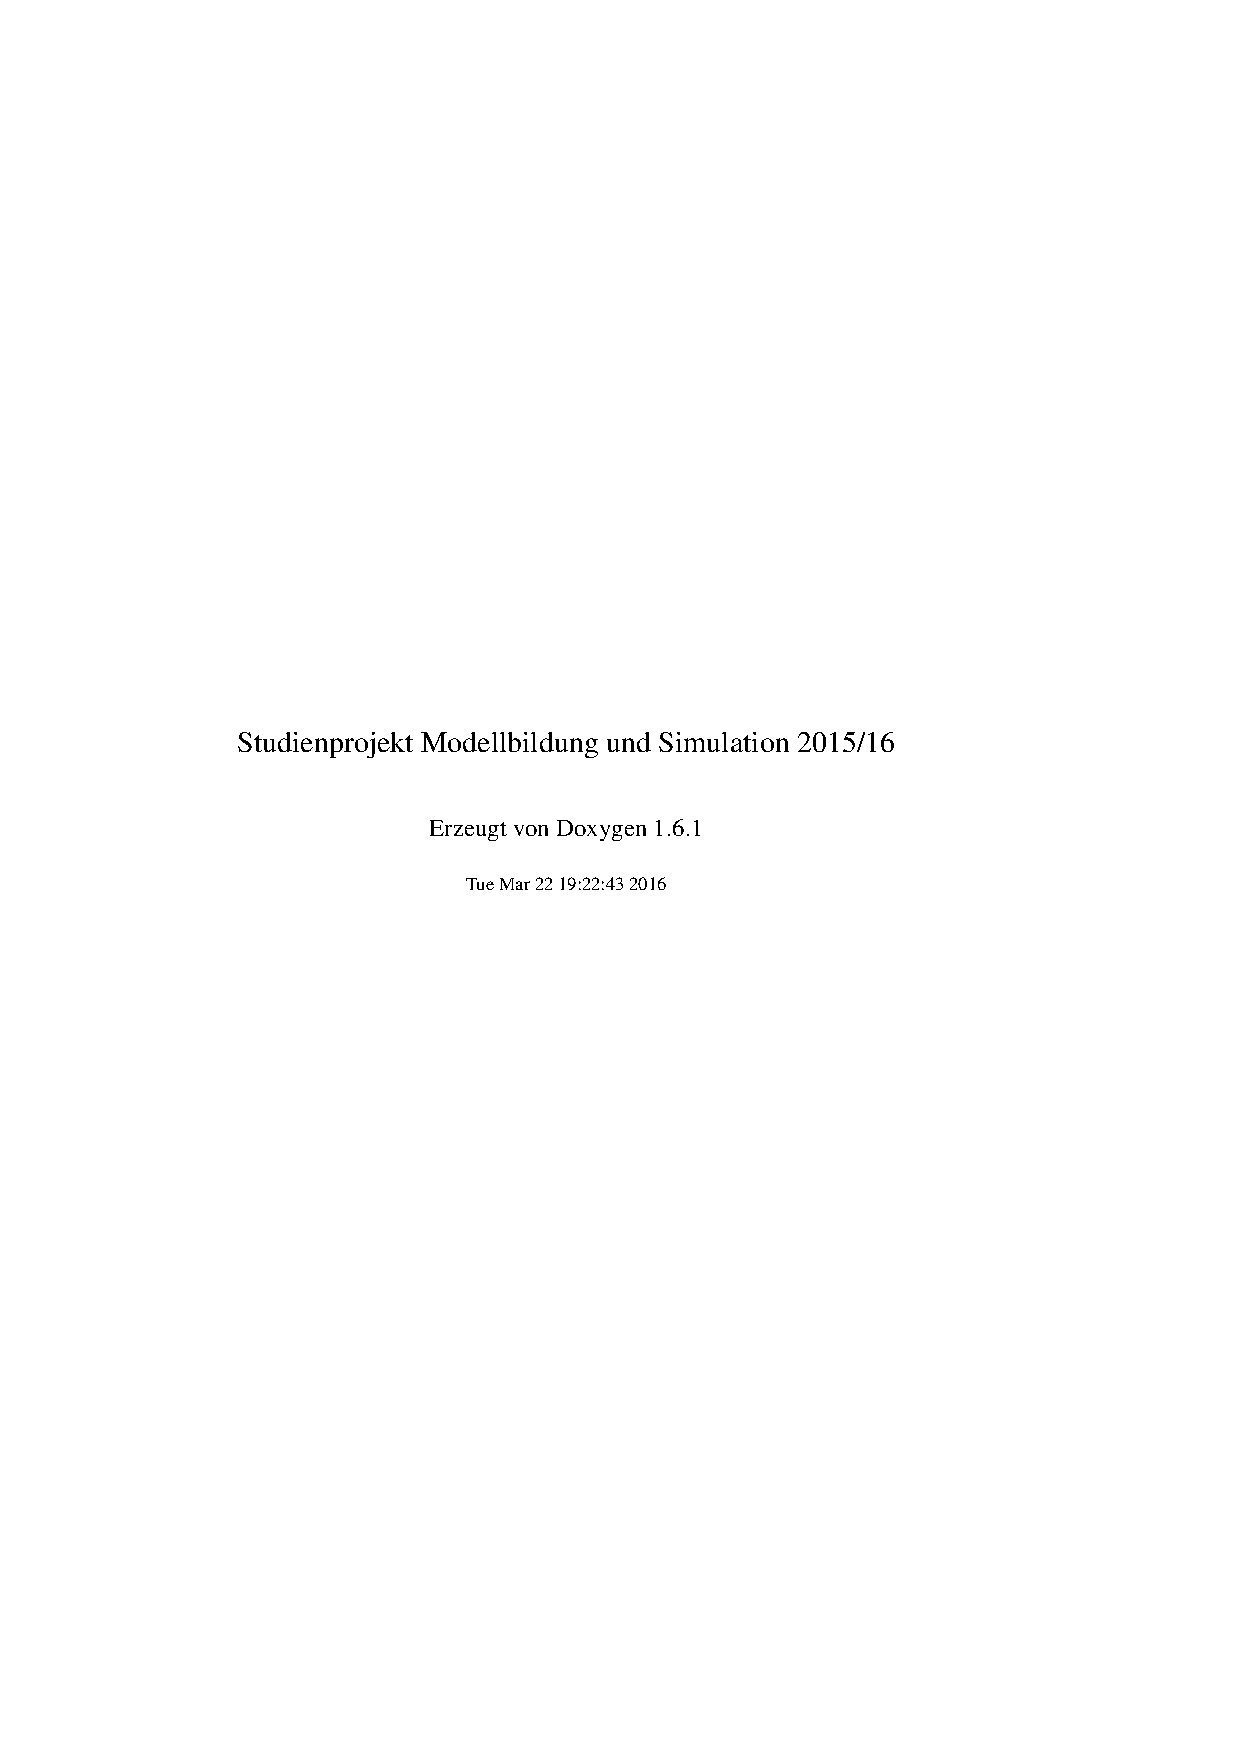
\includepdf{refman.pdf}




\end{document}
